\documentclass[12pt,letter]{article}
\usepackage{geometry}\geometry{top=0.75in}
\usepackage{amsmath}
\usepackage{amssymb}
\usepackage{mathtools}
\usepackage{xcolor} % Color words
\usepackage{cancel} % Crossing parts of equations out
\usepackage{tikz}       % Drawing 
\usetikzlibrary{shapes.geometric, arrows}
\usepackage{pgfplots}   % Other plotting
\usepgfplotslibrary{colormaps,fillbetween}
\usepackage{placeins}   % Float barrier

% Don't indent
\setlength{\parindent}{0pt}
% Function to replace \section with a problem name specifically formatted
\newcommand{\problem}[1]{\vspace{3mm}\Large\textbf{{Problem
{#1}\vspace{3mm}}}\normalsize\\}
% Formatting function, like \problem
\newcommand{\ppart}[1]{\vspace{2mm}\large\textbf{\\Part
{#1})\vspace{2mm}}\normalsize\\}
% Formatting 
\newcommand{\condition}[1]{\vspace{1mm}\textbf{{#1}:}\normalsize\\}

\begin{document}
\title{CIS 551: Assignment 5}
\author{Steven Walton}
\maketitle
\problem{1: 19.2}
Consider a relation $R$ with five attributes $ABCDE$. You are given the
following dependencies. 
\begin{figure}[ht!]
    \center
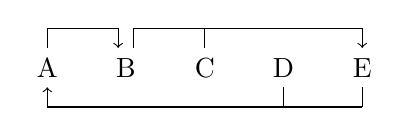
\begin{tikzpicture}
    \node (A) at (0,0) {A};
    \node (B) at (1,0) {B};
    \node (C) at (2,0) {C};
    \node (D) at (3,0) {D};
    \node (E) at (4,0) {E};

    \draw[-] (A) -- (0,0.5);
    \draw[-] (0,0.5) -- (0.9,0.5);
    \draw[->] (0.9,0.5) -- (0.9,0.25);

    \draw[-] (1.1,0.25) -- (1.1,0.5);
    \draw[-] (C) -- (2,0.5);
    \draw[-] (1.1, 0.5) -- (4, 0.5);
    \draw[->] (4, 0.5) -- (4,0.25);

    \draw[-] (E) -- (4, -0.5);
    \draw[-] (D) -- (3, -0.5);
    \draw[-] (4,-0.5) -- (0, -0.5);
    \draw[->] (0,-0.5) -- (0, -0.25);
\end{tikzpicture}
\end{figure}
\ppart{1}
List all keys for R

We can see that $A\rightarrow B$ which means we can rewrite the relationships as
$ACDE$. Giving us

\begin{figure}[ht!]
    \center
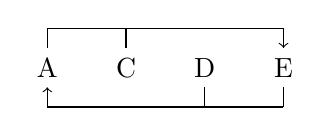
\begin{tikzpicture}
    \node (A) at (0,0) {A};
    \node (C) at (1,0) {C};
    \node (D) at (2,0) {D};
    \node (E) at (3,0) {E};

    \draw[-] (A) -- (0,0.5);
    \draw[-] (C) -- (1,0.5);
    \draw[-] (0, 0.5) -- (3, 0.5);
    \draw[->] (3, 0.5) -- (3,0.25);

    \draw[-] (E) -- (3, -0.5);
    \draw[-] (D) -- (2, -0.5);
    \draw[-] (3,-0.5) -- (0, -0.5);
    \draw[->] (0,-0.5) -- (0, -0.25);
\end{tikzpicture}
\end{figure}

With $A$ and $C$ we are given $E$. Thus we have

\begin{figure}[ht!]
    \center
\begin{tikzpicture}
    \node (A) at (0,0) {A};
    \node (C) at (1,0) {C};
    \node (D) at (2,0) {D};
\end{tikzpicture}
\end{figure}

And we no longer have any relationships.

Similarly we can get the other keys. Giving us the answer:

$ACD$, $BCD$, $CDE$

\ppart{2}
Is R in 3NF?

\part{3}
Is R in BCNF?

\problem{2: 19.6}
Suppose that we have the following three tuples in a legal instance of a
relation scheme $S$ with three attributes ABC (listed in order): $(1,2,3),
(4,2,3), \text{ and } (5,3,3)$.

\ppart{1}
Which of the following dependencies can you infer does \textit{not} hold over
scheme $S$?

(a) $A \rightarrow B$, (b) $BC \rightarrow A$, (c) $B \rightarrow C$

\ppart{2}
Can you identify any dependencies that hold over $S$?

We are only given an instance of $S$ and can't determine what relationships hold
for all instances of $S$.

\problem{3}
Removed from assignment

\problem{4}
Consider relation $R = ABCDE$ with the below relationships. Convert to BCNF.

\begin{figure}[ht!]
    \center
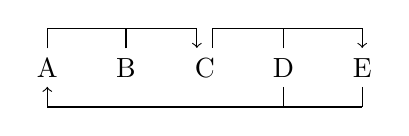
\begin{tikzpicture}
    \node (A) at (0,0) {A};
    \node (B) at (1,0) {B};
    \node (C) at (2,0) {C};
    \node (D) at (3,0) {D};
    \node (E) at (4,0) {E};

    \draw[-] (A) -- (0,0.5);
    \draw[-] (B) -- (1,0.5);
    \draw[-] (0,0.5) -- (1.9, 0.5);
    \draw[->] (1.9,0.5) -- (1.9, 0.25);

    \draw[-] (2.1, 0.25) -- (2.1, 0.5);
    \draw[-] (D) -- (3, 0.5);
    \draw[-] (2.1, 0.5) -- (4, 0.5);
    \draw[->] (4,0.5) -- (4, 0.25);

    \draw[-] (D) -- (3, -0.5);
    \draw[-] (E) -- (4, -0.5);
    \draw[-] (4,-0.5) -- (0, -0.5);
    \draw[->] (0, -0.5) -- (A);
\end{tikzpicture}
\end{figure}

\problem{5: 19.13}

\problem{6}
Let $R$ be a relation, $X$ a set of attributes of $R$, and $A$ an attribute of
$R$. (Also denote that $XA$ the result of adding $A$ to $X$) Define the support
of $X$, written as $\#X$, as the number of distinct tuples in $R|X$ ($R$
restricted to, or projected onto, the attributes of $X$). Prove that if $X
\rightarrow A$, then $\#X = \#XA$.

\problem{7}
Prove that if $R$ is in 3NF and has only one candidate key, then $R$ is in BCNF.

\problem{8}
Insert the following values into an initially empty B+ tree with parameter $d=2$
and values $17, 11, 50, 22, 5, 35, 42, 60, 15, 30, 25, 27, 37, 40, 20$.

\problem{9}
Repeat the previous problem with $d=3$

\problem{10: 10.8 part 1}
Assume that you have just built a dense $B+$ tree index using Alternative (2) on
a heap file containing 20,000 records. The key field for this $B+$ tree index is
a 40-byte string, and it is a candidate key. Pointers (le., record ids and page
ids) and (at most) 10-byte values. The size of one disk page is 1000 bytes. The
index was built in a bottom-up fashion using the bulk loading algorithm, and the
nodes at each level were filled up as much as possible.

\ppart{1}
How many levels does the resulting tree have?


\end{document}
